\documentclass[12pt]{article}
\usepackage[hmargin={1in},vmargin={1in,1in},foot={.6in}]{geometry}   
\geometry{letterpaper}       
%\geometry{landscape}          
%\usepackage[parfill]{parskip}
\usepackage{color,graphicx}
%\usepackage{covington}
%\usepackage{xyling}
\usepackage{setspace}
\usepackage{amsmath}
\usepackage{amssymb}
%\usepackage{graphicx,color}
%\usepackage{theorem}
%\usepackage{tabularx}
%\usepackage{subfig}
%\usepackage{vowel}
%\usepackage{mathrsfs}
\usepackage{varioref}
\usepackage{textcomp}
%\usepackage{avm}
\usepackage{textcomp}
\usepackage{mflogo}
\usepackage{wasysym}
%\usepackage{pstricks, pst-plot, pst-node, pst-tree, colortab}
%\usepackage{qtree}
 %\usepackage{tree-dvips}
 \usepackage{linguex}
%\usepackage{gb4e}
 \usepackage{multirow}
 %\usepackage[stable]{footmisc}
 \usepackage{pifont}
%\usepackage{todonotes}
%\usepackage{natbib}
\usepackage[normalem]{ulem}
\usepackage{wrapfig}

 %\setlength{\parskip}{.55ex plus 0.1ex}


\usepackage{fancyhdr} % This should be set AFTER setting up the page geometry
\pagestyle{plain} % options: empty , plain , fancy
\lhead{}\chead{}\rhead{}
\renewcommand{\headrulewidth}{.3pt}
\lfoot{}\cfoot{\thepage}\rfoot{}
%\renewcommand{\footrulewidth}{.3pt}
\newcommand{\txtp}{\textipa}
\renewcommand{\rm}{\textrm}
\newcommand{\sem}[1]{\mbox{$[\![$#1$]\!]$}}
\newcommand{\lam}{$\lambda$}
\newcommand{\lan}{$\langle$}
\newcommand{\ran}{$\rangle$}
\newcommand{\type}[1]{\ensuremath{\left \langle #1 \right \rangle }}
\newcommand{\defeq}{$\mathrel{\mathop:}=$ }
\renewcommand{\and}{$\wedge$ }


%\renewcommand{\Extopsep}{2pt}


\newcommand{\bex}{\begin{examples}}
\newcommand{\eex}{\end{examples}}

%bullet points
\newcommand{\bit}{\begin{itemize}}
\newcommand{\eit}{\end{itemize}}

%numbering, non sequential
\newcommand{\ben}{\begin{enumerate}}
\newcommand{\een}{\end{enumerate}}

\renewcommand{\abstractname}{The goal:}


%numbering, what you would use in a paper when you don't want the numbering to stop every time you end an example. 
%\newcommand{\bex}{\begin{enumerate}\setcounter{enumi}{\thesaveenumi}\item{}\begin{enumerate}}
%\newcommand{\eex}{\end{enumerate}\setcounter{saveenumi}{\theenumi}\end{enumerate}}

%%these are the brackets used for writing up semantic meanings 
%\newcommand{\lbr}{\textrm{\textlbrackdbl}}
%\newcommand{\rbr}{\textrm{\textrbrackdbl}}
%\renewcommand{\rm}{\textrm}

%this describes the numbering system (roman vs arabic numerals and so forth)
\renewcommand\theenumi {\alph{enumi}}
\renewcommand\theenumii {\alph{enumii}}
\renewcommand\labelenumi {\theenumi. }
\renewcommand\labelenumii {\theenumii.}
\labelformat{enumi}{(\theenumi)}
\labelformat{enumii}{(\theenumi\theenumii)}
\newcounter{saveenumi}

%\renewcommand{\labelitemi}{\textbf{---}}
%\renewcommand{\labelitemii}{\textbf{$\cdot$}}

%\linespread{1.5}

%\qtreecenterfalse

%\linespread{1}

\begin{document}

\begin{center}\textbf{Property subjectivity predicts adjective ordering preferences}
\end{center}
	
Our approach to the investigation of adjective ordering preferences synthesizes strategies from the psychological approach, probing the principles that underlie these preferences \cite{sweet1898,ziff1960,martin1969determinants,martin1969competence,martin1970,kemmereretal2009}, and from the grammatical approach, using descriptive adjective classes to structure and inform our hypotheses \cite{dixon1982,sproatshih1991,cinque1994,scott2002}. We first conducted a corpus study to measure, for 26 adjectives from seven different classes (size, quality, age, texture, shape, color, material), what their mean distance from the modified noun is in phrases with either two or three adjectives (e.g., ``a nice green color'' or ``some big heavy red cloaks''). We extracted all such cases from the Switchboard corpus, as well as from both the written and spoken portions of the British National Corpus (for a total of 39,199 cases). Mean distance from the noun for each adjective class is shown in Fig.~1.
Conducting pairwise Bonferroni-corrected comparisons between classes on the average distance-from-noun scores calculated in Fig.~1 yields the following ordering preferences, which closely track the previous reports in the literature:
$$ size \geq quality > age > texture > shape > color > material \label{inferred-order-preferences}$$

We closely replicated these inferred ordering preferences in Expt.~1, where we elicited naturalness judgments on adjective-adjective-noun object descriptions, permuting the relative order of the adjectives. Participants indicated which ordering of an adjective-adjective-noun object description sounded more natural (e.g., ``the big red apple'' vs.\ ``the red big apple''). On the basis of these naturalness ratings, we computed for each adjective-adjective pairing its preferred, canonical order. We then determined how often an adjective from a given class occurred first in an adjective-adjective-noun configuration; Fig.~2 plots these average distance scores, where a value of 1 signals that a class's adjectives always occur first in preferred adjective-adjective-noun orderings. 

Having established the robustness of ordering preferences both in production (measured in our corpus experiment) and in comprehension (measured in our rating experiment), we then shifted focus to the source of these preferences. While researchers may disagree about its details, the psychological explorations of ordering preferences converge on the idea that aspects of  adjectives' meaning (i.e., specificity, context-sensitivity, reliance on comparison, etc.) determine their relative order.  Here we distill the proposals that precede us into a single feature, the subjectivity of the property named, as the single best predictor of ordering preferences. 

We conducted Expt.~2 to measure the subjectivity of adjectives and the broader classes to which they belong. Participants evaluated the potential for faultless disagreement between two differing descriptions of an object. For example, an experimental trial would have Mary assert ``that apple is old,'' then have Bob counter with ``that apple is not old.'' To the extent that both Mary and Bob can be right in their descriptions of the apple, ``old'' admits that degree of faultless disagreement. 
Thus, the extent to which two people can disagree about a description without one necessarily being wrong determines the subjectivity of that description. We validated our faultless disagreement measure in a separate paradigm, which explicitly asked about the potential ``subjectivity'' of object descriptions; the results of these two methods were highly correlated ($r^{2} = 0.89$), suggesting that the measures they invoked converge in their estimation of adjective subjectivity.

Fig.~3 plots faultless disagreement ratings for adjectives and their respective classes. Based pairwise comparisons of these aggregate scores, we inferred the following adjective class subjectivity raking:
$$ quality \geq size > texture \geq age > color \geq shape \geq material \label{inferred-subjectivity}$$

To evaluate the predictive power of subjectivity in determining adjective order, we compared acceptability ratings from Expt.~1 with faultless disagreement scores from Expt.\ 2. We first calculated a subjectivity difference score for each class configuration, \textsc{class1} \textsc{class2}, subtracting the average faultless disagreement score for \textsc{class1} from the average faultless disagreement score for \textsc{class2}. Fig.~4 plots class configuration acceptability ratings against faultless disagreement difference scores.

\noindent
\begin{minipage}[t]{.48\linewidth}
	\vspace{0pt}
	\begin{center}
		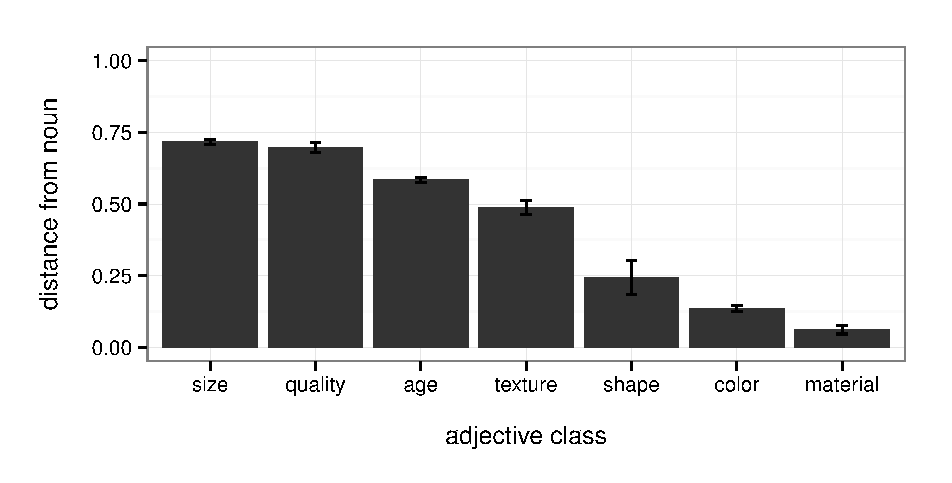
\includegraphics[width=\linewidth]{plots/corpus_distance_plot.eps}
	\end{center}
	\vspace{-15pt}
	Fig.~1 (corpus results): Average distance from noun by adjective class for cases with at least two modifying adjectives.
	\begin{center}
		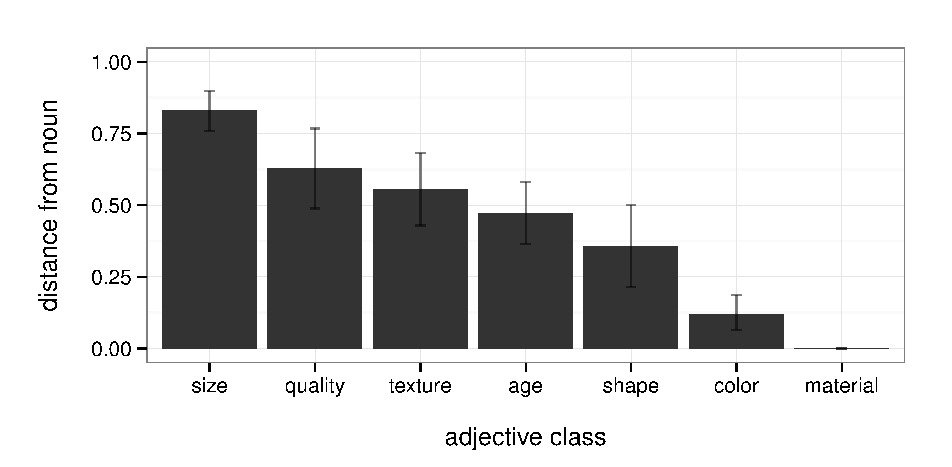
\includegraphics[width=\linewidth]{plots/class_distance_by_adj.eps}
	\end{center}
	\vspace{-15pt}
	Fig.~2 (Expt.~1 results): Average preferred distance from noun for each adjective class.
	\begin{center}
		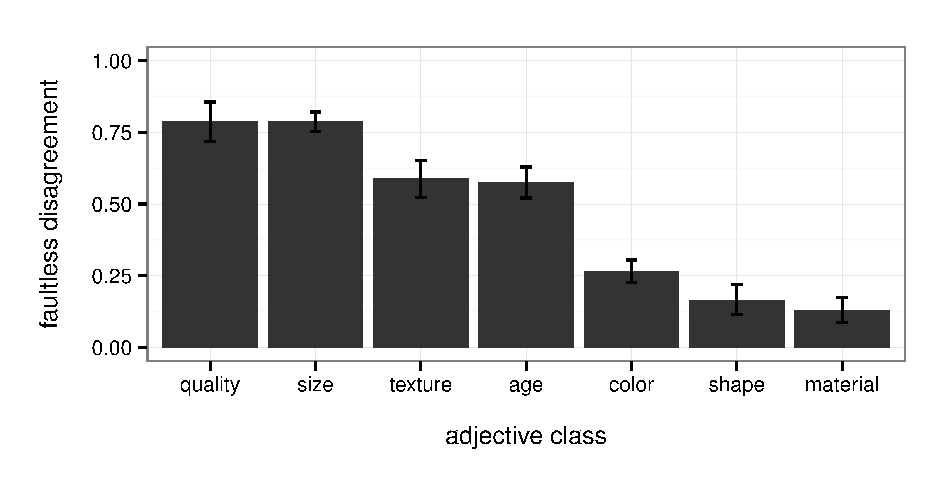
\includegraphics[width=\linewidth]{plots/faultless_class_plot.eps}
	\end{center}
	\vspace{-15pt}
	Fig.~3 (Expt.~2 results): Average faultless disagreement scores for adjectives by class.
\end{minipage} \hfill
\begin{minipage}[t]{.48\linewidth}
	\vspace{0pt}	
	\begin{center}
		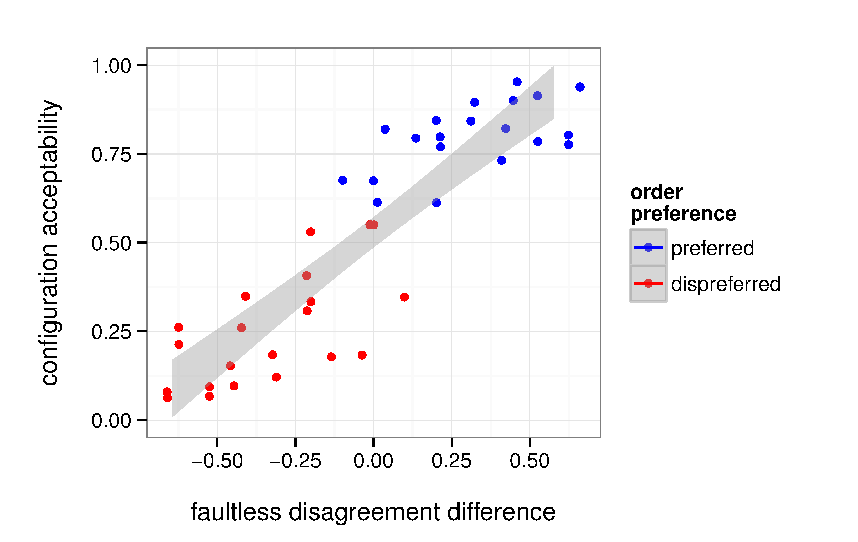
\includegraphics[width=\linewidth]{plots/faultless_order_preference.eps}
	\end{center}
	Fig.~4: Class-level order preferences plotted against difference in faultless disagreement between A1 and A2 (values greater than 0 indicate that the more subjective adjective class occurs farther from the noun).
\end{minipage}


\newpage

\begin{thebibliography}{10}
	\bibitem{chomsky1965}
	N.~Chomsky, {\em Aspects of the Theory of Syntax} (1965).
	
	\bibitem{sweet1898}
	H.~Sweet, {\em A New English Grammar} (1898).
	
	\bibitem{bloomfield1933}
	L.~Bloomfield, {\em Language} (1933).
	
	\bibitem{sproatshih1991}
	R.~Sproat and C.~Shih, 1991. {\em The cross-linguistic distribution of adjective ordering restrictions}, Interdisciplinary approaches to language: Essays in honor of S.-Y.~Kuroda (1991), pp.~565--593.
	
	\bibitem{martin1969competence}
	J.~E.~Martin, {\em Some Competence-Process Relationships in Noun Phrases with Prenominal and Postnominal Adjectives}, Journal of Verbal Learning and Verbal Behavior, 8 (1969), pp.~471--480. 	
	
	\bibitem{wulff2003}
	S.~Wulff, {\em A multifactorial corpus analysis of adjective order in English},
	International Journal of Corpus Linguistics, 8 (2003), pp.~245‒-282.
	
	\bibitem{ziff1960}
	P.~Ziff, {\em Semantic Analysis} (1960).
	
	\bibitem{martin1969determinants}
	J.~E.~Martin, {\em Semantic Determinants of Preferred Adjective Order}, Journal of Verbal Learning and Verbal Behavior, 8 (1969), pp.~697--704. 
	
	\bibitem{martin1970}
	J.~E.~Martin, {\em Adjective Order and Juncture}, Journal of Verbal Learning and Verbal Behavior, 9 (1970), pp.~379--383. 
	
	\bibitem{haiman1985}
	J.~Haiman, {\em Natural Syntax} (1985).
	
	\bibitem{dixon1982}	
	R.~M.W.~Dixon, {\em Where have all the adjectives gone?, and other essays in semantics and syntax} (1982).
	
	\bibitem{cinque1994}
	G.~Cinque, {\em On the evidence for patial N-movement in the Romance DP}, Paths towards Universal Grammar. Studies in honor of Richard S.~Kayne (1994), pp.~85--110.
	
	\bibitem{scott2002}
	G.-J.~Scott, {\em Stacked adjectival modification and the structure of nominal phrases}, The Cartography of Syntactic Structures (2002), pp.~91--120.
	
	\bibitem{rohde2005}
	D.~Rohde, TGrep2 User Manual (2005).
	
	\bibitem{degenjaeger-tdt}
	J.~Degen and T.F.~Jaeger, The TGrep2 Database Tools (2011).
	
	\bibitem{godfrey1992}
	J.~Godfrey and E.~Holliman and J.~McDaniel, {\em Switchboard: A Telephone Speech Corpus for Research and Development}, Proceedings of ICASSP-92 (1994),
	pp.~517--520.
\end{thebibliography}


%\bibliographystyle{chicago}
%\bibliography{greg.bib}




\end{document}